%%%%%%%%%%%%%%%%%%%%%%%%%%%%%%%%%%%%
% This is the template for submission to MICRO 2019
% The cls file is modified from 'sig-alternate.cls'
%%%%%%%%%%%%%%%%%%%%%%%%%%%%%%%%%%%%

\documentclass{sig-alternate}
\usepackage{mathptmx} % This is Times font

\usepackage{fancyhdr}
\usepackage[normalem]{ulem}
\usepackage[hyphens]{url}
\usepackage[sort,nocompress]{cite}
\usepackage[final]{microtype}
\usepackage{flushend}
% Always include hyperref last
\usepackage[bookmarks=true,breaklinks=true,letterpaper=true,colorlinks,linkcolor=black,citecolor=blue,urlcolor=black]{hyperref}




% Packages and commands not in template
\usepackage[dvipsnames]{xcolor} %color package
\usepackage{pifont} %check and x font
\newcommand{\cmark}{\textcolor{ForestGreen}{\ding{51}}}%
\newcommand{\xmark}{\textcolor{red}{\ding{55}}}%




% Ensure letter paper
\pdfpagewidth=8.5in
\pdfpageheight=11in

%%%%%%%%%%%---SETME-----%%%%%%%%%%%%%
\newcommand{\microsubmissionnumber}{580}
%%%%%%%%%%%%%%%%%%%%%%%%%%%%%%%%%%%%

\fancypagestyle{firstpage}{
  \fancyhf{}
  \renewcommand{\headrulewidth}{0pt}
  \fancyhead[C]{\vspace{15pt}\normalsize{MICRO 2019 Submission
      \textbf{\#\microsubmissionnumber} -- Confidential Draft -- Do NOT Distribute!!}} 
  \fancyfoot[C]{\thepage}
}

\pagenumbering{arabic}

%%%%%%%%%%%---SETME-----%%%%%%%%%%%%%
\title{Register File Cache: Efficient Memory Disambiguation and Pipeline Prefetching} 
%%%%%%%%%%%%%%%%%%%%%%%%%%%%%%%%%%%%

\begin{document}
\maketitle
\thispagestyle{firstpage}
\pagestyle{plain}




\begin{abstract}
{\color{red} Recent load value prediction techniques improve IPC by predicting load addresses and prefetching the data into the pipeline. This achieves the same zero load-to-use latency as an all-instruction value predictor but with simpler CPU components making more feasible to implement in hardware. However, it comes with a great increase in pressure in the physical register file and L1 cache in order to validate predictions. %Register reuse techniques could help mitigate the problem by providing load-to-load forwarding, but as we show in this work, state-of-the art register reuse techniques only take minimal advantage of the reuse potential.

In this work, we make two observations: (1) the value predicted address are special and that the validation of most predicted addresses do not require the load to be replayed to validate the prediction, most of the CPU components required to validate the predicted load are already present in the CPU to detect memory ordering violations; and (2) due to having addresses early in the pipeline, we can easily cache, manage and detect data reuse, and perform load-to-load forwarding through the physical register, further decreasing register and cache pressure. %The address prediction components provided by load value predictors solves this issue by making load addresses available at decode and allows for a more effective register reuse detection and forwarding technique since it is based on load addresses, i.e. the same strategy used in any other cache level in the memory hierarchy.

Our proposed address based register reuse technique improves data forwarding through the register file by XX\% on average (up to XX\%) compared to a state-of-the-art register sharing strategy, and reduces L1 accesses by YY\% (up to YY\%) compared to a stand alone load value predictor without losing any performance improvements provided by the same load value predictor. Moreover, the strategy has minimal storage overheard since it leverages the components required by load value predictors and memory ordering violation detection to detect and safely reuse data in the register file.
}

\end{abstract}




\section{Introduction}
%Single thread performance is still imperative in modern applications and CPU architectures need keep improving in this area. 
Satisfying loads as early as possible is of critical importance to performance. Not surprisingly, a plethora of micro-architectural techniques have been proposed towards this purpose. Unfortunately, in many cases, achieving the desired effect with a technique also means undesired consequences, e.g.,: comprimizing energy efficiency or exerting increased pressure onto the memory system. 
In this paper, we re-revisit the interface of the core to the cache hierarchy (i.e., L1). We are not concerned on how to reduce the number of cache misses or the cost of each miss ---more generally the mean time to access memory--- as these are orthogonal to our work. What we are concerned here is to optimize the latency starting from accessing data in L1 all the way to using such data in a load-dependent instruction. We aim to view the problem from a new perspective: Satisfy as many loads as we can, as early as possible, by: i) making the best use of the mechanisms and datapaths that already exist in a typical out-of-order microarchitecture; ii) adding as little as possible in terms of helper structures, and iii) avoiding overtaxing other resources such as the ports to the L1.

Historically, one point of attack for the problem of load latency has been to bring the cache hierarchy inside the core in the form of a faster L0~\cite{}. However, this does not fundamentally change the way we satisfy loads.  Loads still have to generate their effective address and access the L0 in the address name space.

A more radical approach is to use value prediction (VP)~\cite{lipasti-shen, others more recent}. VP tries to guess the result of an instruction. In the case of a load, VP predicts the value loaded. Overall, VP allows instructions to proceed with predicted operands without waiting for the instructions that create these operands to execute. This \emph{speculatively} breaks true data dependencies and thus has the potential to increase instruction level parallelism (ILP) beyond the dataflow limit.
While promising, this technique comes with the caveat that mispredictions are costly so predicted values are only used when the prediction has a high confidence. This results in low coverage. Furthermore, since stores change the values in memory, they can interfere with predictions. This further decreases confidence in the prediction (and in coverage).
Load VP circumvents both the address name space and the register name space, predicting values and writing them directly into the destination register or forwarding them to waiting dependent instructions. However, as a prediction, VP needs to validate the predicted value by comparing it with the value accessed through the address name space. This means that a value-predicted load will execute and access the L1 and compare its loaded value to the predicted value. 
 
Sheikh et al. make the observation that addresses are easier to predict than data, and propose the \textit{Decoupled Load Value Prediction} (DLVP) technique that predicts the load addresses instead of the load values and prefetches the data into the pipeline just in time to be consumed by the dependent instruction(s). This effectively achieves the same zero load-to-use latency of a value-predicted load, but with increased coverage for load instructions, fewer number of iterations to trust the prediction, and fewer mispredictions due to stores changing the predicted value (mispredictions still occur when the store is out-of-order with respect to the access of the value but that is a more rare occurrence than the mispredictions of a value-prediction approach).
While effective this technique also significantly increase accesses to memory since every predicted load address needs access the memory twice, once to prefetch and a second to validate the result in case of coherence or memory ordering violation. 
In contrast to value prediction, address prediction still maintains the connection to the address name-space, loading actual values from the predicted memory addresses.

In contrast to VP and DLVP, \emph{register sharing} techniques work in the \emph{register name space}. In these techniques the address name space is used to establish a connection between instructions that effectively access the same address and instead of communicating via the cache hierarchy where the values are mapped on their respective memory addresses, they communicate via the register file where an address is \emph{mapped} after being loaded into a register.
The seminal example is the speculative cloacking and bypassing technques by Moshovos and Sohi~\cite{moshovos98}, where a connection is established via the address name space, between a load that is memory-dependent on an earlier store. Communication between future instances of the store and the load is then \emph{speculatively} routed via the register file as soon as the store-value is available (without the need to compute the addresses). There is no need to access the actual value from the address name space (assuming the value can only change by stores of the same thread), but the addresses of the store and the load are eventually  compared to verify the speculation. 

Things are more complicated for register-sharing techniques that concern connections between loads, i.e., establishing a connection in the register name space between loads that access the same address. The complication here is that (in case of loads) we are unaware what our own stores are doing (let alone remote stores from other cores that make their presence known via invalidations). This means that establishing a connection between loads will eventually require \emph{value validation}: all loads must load their value in the correct order and verify that the value they received speculatively was correct---validating that they used the same address is not enough.

%Moreover this technique misses one great advantage of having addresses early on in the CPU pipeline, which is the ability to take advantage of temporal and spacial data locality available in memory.

In this work we make the observation that predicting addresses enables us to do more than increase value prediction coverage. By using addresses we're able to validate most predictions without having to the re-execute the load instructions, since we can detect most memory violations using addresses alone, reducing register and L1 pressure; and we can detect data temporal reuse naturally and manage it in the register file, reducing register and L1 pressure even further and beyond state of the art register sharing techniques. Since applications also expose a great degree of spacial reuse, in some cases we're even able to expose more locality than the theoretical maximum available in the window provided by the load queue. 

Our technique shows an improvement of xx\% bla bla bla.


%\begin{figure}[ht]
%\centerline{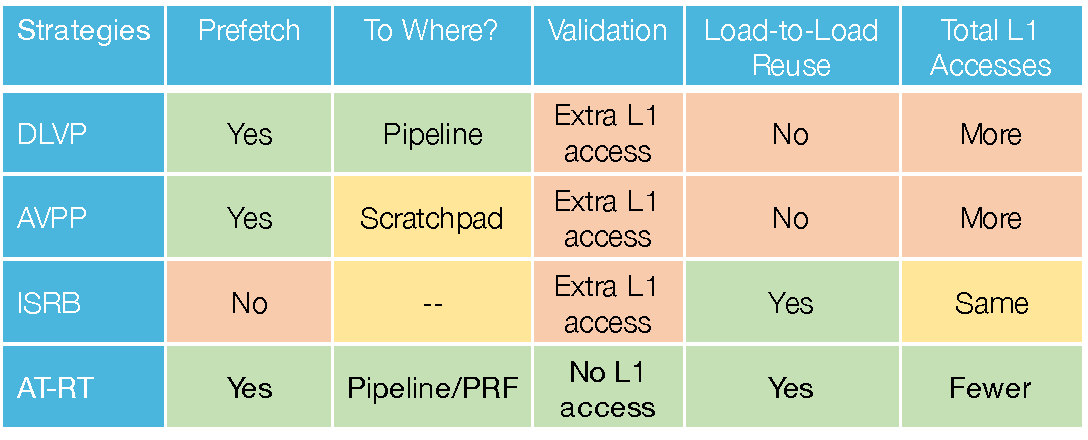
\includegraphics[width=0.50\textwidth]{diagrams/VsTable.pdf}}
%%\captionsetup{justification=centering}
%\caption{Table motivating our work}
%\label{fig:DistVsValue}
%\end{figure}

\begin{scriptsize}
%\begin{table}[h!]
\begin{table*}[h!]
  \centering
  \begin{tabular}{|c|c|p{20mm}|p{20mm}|p{25mm}|p{20mm}|p{10mm}|p{20mm}|}
    \hline
    \textbf{Strategies} & 
    \textbf{Prefetch} & 
    \textbf{Granularity} & 
    \textbf{To Where?} &
    \textbf{Load-Load reuse} & 
    \textbf{Validation} & 
    \textbf{L1 accesses} & 
    \textbf{comment}\\
    \hline
    
    \hline
    DLVP~\cite{} &  \cmark & {\color{orange}accessed \newline item (e.g., word)} & pipeline & \xmark &  {\color{red} Value-based} &  {\color{red} more} &    \\
    \hline
    AVPP~\cite{} &  \cmark & {\color{green}block} \newline (e.g., 128 bits) & scratchpad \newline (L0)  & \xmark & {\color{red} Value-based} &  {\color{red} more} &   \\
    \hline
    ISRB~\cite{} &  \xmark & -- & -- & \cmark ({\color{orange}single address} / {\color{green}multiple loads}) & {\color{red} Value-based} &  {\color{black} same} &    \\
    \hline
    AT-RT~\cite{} &  \cmark & {\color{green}block} \newline (e.g., 128 bits)& pipeline/PRF & \cmark ({\color{green}multiple addresses} / {\color{green}multiple loads}) &  {\color{green} Address-based} & {\color{green} fewer} &    \\
    \hline

    
    \hline
  \end{tabular}
  \caption{Comparison of }
  \label{table:formatting}
\end{table*}
\end{scriptsize}




























\section{Background}

\subsection{Register sharing}
Register sharing was originally proposed by Jourdan et al.~\cite{} to achieve register move elimination. The mechanism detects reuse between instructions and tracks the lifetime of the shared data with registers reference counters. Several efforts have been proposed to make the tracking and sharing of registers more efficient, Perais et al.~\cite{} in particular proposed \textit{Inflight Shared Register Buffer}(ISRB)~\cite{} to improve reuse detection, simplify the tracking of the registers, but also allows for load-to-load data forwarding through the PRF. However, forward data from loads still needs validation by accessing the cache and comparing the values.

While register sharing techniques for register move elimination are orthogonal to our implementation, ISRB does also allow for load-to-load reuse prediction and forwarding which overlaps with our proposal. Give this situation, we will compare our proposal with ISRB as well.

\subsection{Detecting memory ordering violations}
Memory ordering violations can come into forms: (1) internal, where a load incorrectly bypasses and dependent older store; and (2) external, due to memory consistency model violation in the form of coherence invalidation requests.

Internal memory violations happen because, performance-wise, it is important for loads to bypass independent stores. However, bypass needs to happen at issue time where addresses are not yet available so a load is predicted to or not to be dependent on an older store, and speculatively bypassed. If the prediction is incorrect, the loads and their dependency chain need to be replayed. External memory ordering violations can occur due inconsistent  memory ordering and is reverted in the form of external coherence checks. Even if no misprediction happened within the core, the order of memory request might still violate the consistency model due to other memory requests happening in parallel in other CPU cores.

A natural way to solve this issue is to re-execute every speculative load and compare the new result of the load with the previous one to detect if no memory ordering violation happened. This comes with excessive accesses to memory which can have a significant impact in performance and energy, so modern strategies validate most memory bypassing and coherence while minimizing the replaying of loads. For detecting internal violations, NoSQ~\cite{} employs a strategy based on \textit{Store Vulnerability Window} (SVW) and can filter most of the replays (less than 1\% of the instruction needs replaying~\cite{}).

To detect external memory violations, both load and store-queues of the CPU hold the physical address of their respective load or store instructions. Both structures are exposed to coherence traffic and invalidation requests that match any load/store address will be squashed and replayed. The virtual address are also stored in both these queues to facilitate store-to-load forwarding and detection of internal memory ordering violation since they are available sooner than physical addresses, it reduces the penalty of mispredictions.     

\subsection{Value-prediction}
Value prediction techniques can be divided into two classes, computation-based (such as stride predictors~\cite{}) and context-based (such as VTAGE~\cite{} and DVTAGE~\cite{}).  Orosa et al.~\cite{} recently proposed an hybrid that  merges a stride predictor with DVTAGE to improve on both.   

Predicting load values is a better alternative for two reasons, (1) addresses are easier to predict increasing converge; and (2) since only about 25\% of the instructions are loads, the predictor only has to store and predict values for 25\% of the instructions, making the value prediction mechanism smaller and less complex. Recent work on load address only value predictors have shown than predicting only load addresses achieves the same performance benefit as prediction all values~\cite{}.
































\section{Pipeline prefetch, register-sharing shortcomings}
Value predictors require the instruction which had its value predicted to be executed to validate the prediction. In the case of of load instructions, that means executing the load, fetching the data from memory, and compare the memory value with the predicted value. If they are equal, the prediction is deemed correct, if not, the instruction and its dependency chain is replayed. 

Address value predictors, guess the address and prefetches the value instead of guessing the value itself. However, the prediction validation method is the same and thus requires the memory to be accessed again. This means that and address value predictor requires two memory accesses for each prediction, one to prefetch the data and a second to validate the prediction. This can significantly increase the memory accesses of the application if one expects a lot of addresses to be predicted. As expected, address value prediction will be the most effective when as many predictions as possible are made, so current and future implementations of the technique will aim to improve coverage and only compound the problem. Figure ~\ref{fig:} shows the percentage of loads predicted and executed twice, i.e. the percentual increase in memory accesses compared to a traditional non-value predicting pipeline.

Load-to-load forwarding can mitigate this problem. One approach for forwarding, is to store the results of the loads in a intermediate storage~\cite{} and validate the forwarding prediction from there. This is a similar strategy as having a filter-cache/L0 which require extra data storage and data to be written to it. The strategy can perform well on applications with good locality, but have significant negative performance and energy impact when there is not enough locality~\cite{}.  

Alternatively, one can take advantage of register sharing techniques to do load-to-load forwarding using the physical register file, which does not require extra data to be installed. Data is forwarded using the same physical register and only a single memory access needs to be done to validate the forwarded data. However, this strategy requires a high reuse detection ratio to be effective and, as figure~\ref{} shows, the technique is only able to explore a small percentage of the load-to-load forwarding potential expose the load queue window.

While address value prediction is an effective IPC improvement technique, it comes with added pressure on cache and register file since it requires accessing both structures on prefetch and validation. Register file sharing can help mitigate the problem by recycling registers instead of prefetching and only accessing the cache for validation. However, this strategy is only able to cover a small percentage of loads. Even if coverage of perfect, it would only be able to match a non value-predicting pipeline memory accesses since all loads need to access the memory for validation.  

Our proposal leverages the fact the predicted loads have their address available as early as in the fetch stage, and as such, it is possible to have the physical register file behave like a cache for this subset of load instructions -- i.e. detect data load-to-load reuse to avoid extra access to L1 and replication of data in the register file; and validate forwarding with minimal accesses to higher cache levels (in this case, the L1).

%validates all predictions without requiring the second access to memory, effectively removing all validation memory accesses from the address value predictor. And by combining the new validation technique with register file sharing we are also able to remove some of the prefetch requests by forwarding the data from the register file, reducing the total memory accesses even than a standard on address predicting pipeline. Since we use the predicted addresses to detect reuse and forwarding potential, our solution also significantly increases the reuse potential available in the pipeline, reducing pressure in the register file and cache even further. 


























\section{Efficient pipeline prefetching using the PRF as a cache}
To efficiently prefetch into the pipeline using the physical register file, one should aim to turn the PRF into a cache as much as possible. This means we should be able to forward data from the register file if the data is present (no extra data movement within the PRF), and be able to correctly and safely provide the data without accessing extra cache levels. Existing register reusing techniques can be used in an effort to achieve this, but only avoid the problem of the extra data movement (since they still require accessing the L1 for correctness), and even so, they have limited coverage of the total load-to-load reuse potential available.

To effectively use the PRF as a cache we need to address these two issues.

\subsection{Forwarding through register file}
To detect register reuse and perform load-to-load forwarding through register renaming, we propose the introduction of a register reuse table. This table is directed mapped and each entry holds a register ID, a valid bit and a tag. The table is index using the predicted address for each load, since this can be provided by the load value predictor as early as in the fetch stage. On first access, since no entry is invalid, the load instructions go thought the normal renaming path, allocating a destination register. After a register is allocated, they record an entry in the the register renaming table with the register id. When a following load instruction matches on a valid entry with its predicted address, the load instruction can skip allocating a new destination register and use the one in the reuse table. All predicted loads are inserted in the load queue with their respective predicted address. This step is essential to facilitate efficient memory ordering violation detection, i.e. no extra accesses to the register file or redundant accesses to L1.



Each entry also holds the sequence number of the last loads that indexed it to deal with memory ordering issues (further discussion ahead).

\subsection{Forwarding validation}
\begin{figure}[ht]
\centerline{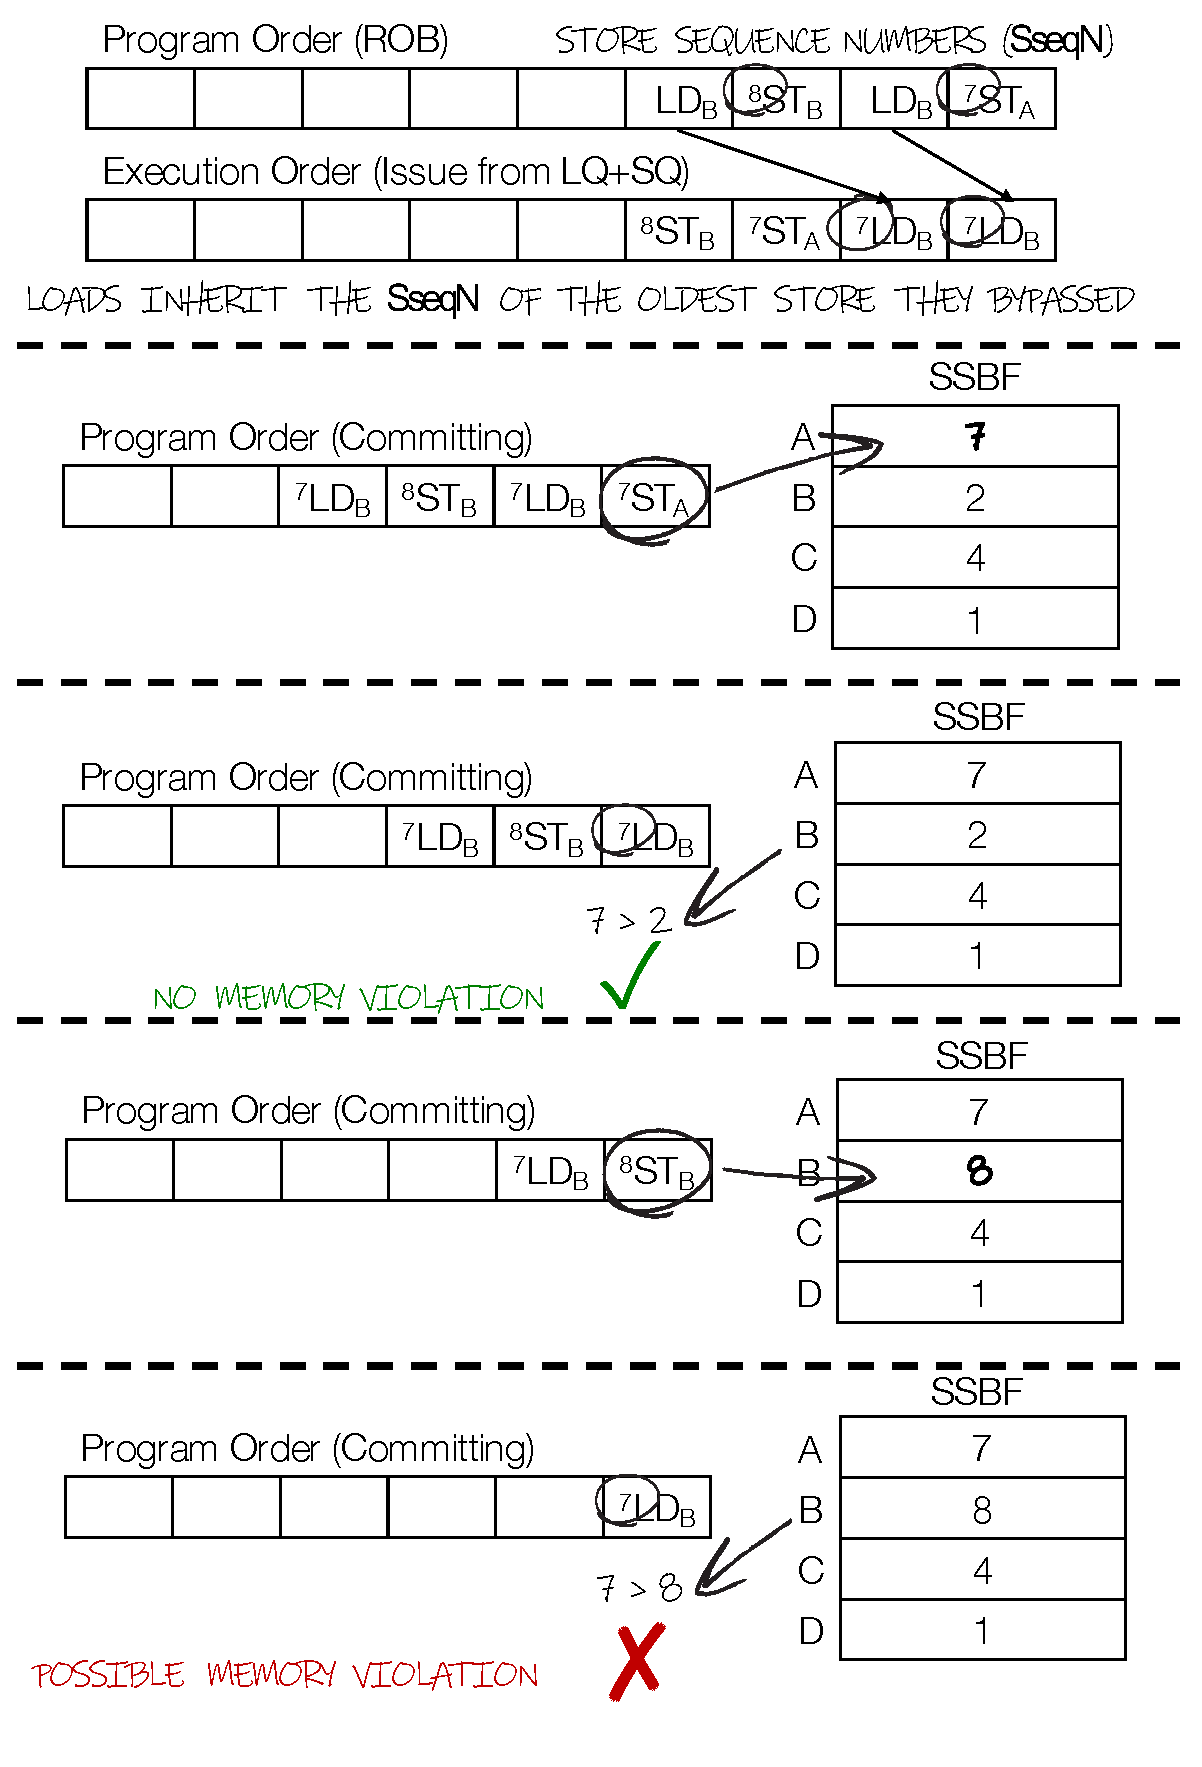
\includegraphics[width=0.50\textwidth]{diagrams/MemOrdValidation.pdf}}
\caption{Example of how the Store Sequence Bloom Filter (SSBF) is used to detect possible memory ordering violations just using Loads/Stores addresses (the letters) and store-sequence-numbers (the numbers)}
\label{fig:MemOrdValidation}
\end{figure}



There are two types of predictions being made in this forwarding strategy: (1) the load address that is produced by the value predictor, and (2) that the load-to-load forwarding does not violate memory ordering, i.e, no conflicting store between them, either from the same CPU or others. The first prediction can be easily validated by computing the address and comparing it to the predicted value. The computed address still needs to be translated to avoid synonyms and verify page permissions, so an access to the TLB is still required. This is however not a problem since modern architectures implement multiple level TLBs, with the the first level being directed mapped and at least one order of magnitude smaller than the L1, making its dynamic energy usage inconsequential~\cite{}. Since the predicted address is stored in the load queue, no extra access to register file is required to fetch the predicted address for comparison and validation.

Validating the memory ordering is a bit more difficult and needs to be separated into two different types, external and internal. External ones comes in the form of memory coherence invalidation requests. Although complex to solve, this type of ordering violations are present in any multi-core micro-architecture as well and as such, the CPU must already have mechanism to detect the violating loads~\cite{}, rollback the values of the shared registers~\cite{} and replay the infringing instruction chains~\cite{}. The only extra step introduced by our mechanism is that the register reuse table also needs to be accessed to invalidate the entry for that address. Since the table is directed mapped and indexed by addresses, this is a fast access to zero the valid bit. Is also relevant to mention that this negative coherence interaction can be completely avoided by delaying coherence requests in L1 without any loss of performance~\cite{}.

In order to deal with internal memory ordering problems, it is required for our mechanism to interact with the memory dependency predictor. While our solution is independent of the memory dependency predictor used, we still need to chose one for modeling. We chose the one proposed bu A. Roth~\cite{} since it minimises redundant accesses accesses to L1 to validate memory ordering by filtering loads that are not in a \textit{store venerability window} (SVW). This mechanism relies on \textit{store sequence numbers} (SseqN) to detect if a load is in the venerability window of a store and only loads that are in the venerability windows need to be replayed. This strategy can be naturally extended to any register reuse mechanism, by having loads inheriting the SseqN of their forwarded loads and thus inheriting their venerability window as well. %This has implications on the memory bypassing predictor which we will discuss next. 
Again, this is a requirement for any load-to-load forwarding technique, not just the register file based one proposed in this paper. The extra step introduced by our technique is for the register reuse table to be updated accordingly. When a store instruction is at the commit stage, it also needs to index the register reuse table and invalidate the corresponding entry so that the following load that match that same address do not forward the stale data from older loads.



\subsection{Interaction with the memory bypass predictor}
Both the standalone address based predictor and any load-to-load forwarding techniques need to be informed by speculative memory bypassing (SMB) predictor. Even if there is no correctness issue due to incorrect scheduling, mispeculations can still have a profound impact in performance~\cite{}, requiring the pipeline to be flushed and instruction dependency chains to be replayed. For our solution we use the same load store conflict detector (LSCD) strategy as DLVP~\cite{} to enable or disable forwarding for particular loads before rename. Perais at al.~\cite{} goes one step further and breaks memory dependencies by identifying the producer of a load and renaming the destination register of the load as the source register of the producing store. This effectively allows for load-to-store forwarding through the register file but we do not consider those in this work.  


\subsection{Address prediction}
Even though our solution is independent of the value predictor chosen, we still need to implement one since we require load addresses early in the pipeline to manage register sharing and provide load-to-load forwarding through PRF. As discussed before, there are several classes of value predictors that vary in complexity and accuracy. For simplicity we chosen to implement a stride based predictor~\cite{}. Figure~\ref{} shows the accuracy of our prediction and the predictor details are described in section~\ref{sec:Results}. 

Although very accurate~\cite{}, a stride predictor is not be most accurate one (the most accurate being a hybrid DVTAGE+Stride value predictor~\cite{}). However for our analysis the stride predictor was accurate enough and we feel it provides a good baseline to validate our strategy. It is important to note that more complex and sophisticated value predictors would only increase coverage of loads predicted and/or decrease errors, improving our proposed solution even further.  





















%Coarse grain tags, to track 128-bit/sub-array-width chunks
\section{Expose Spacial Locality in PRF}
Another important function of caches is that they expose spacial locality. While this is desirable for any cache hierarchy level, it seems unnecessary to do the same in the PRF when used in conjunction with DLVP and register sharing. The performance benefit of having the spacial adjacent data already in the "cache level" before needed, is nullified by the prefetching of DLVP. Moreover, the DLVP technique minimises cache pollution, since it will only fetch the data that it predicts it will be used instead of fetching and installing adjacent data (cache line granularity) on every access regardless of reuse.

There is however the possible benefit of reducing total accesses to memory, improving energy efficiency. Unlike L2 and L3s that exchange data at fixed "cache-line" size blocks, L1s are optimised for small and variable data size granularity. Modern vector-load enabled CPUs can have busses to L1 as wide as 512-bits, to be able to satisfy large vector load instruction in a single access. While the performance benefit of supporting such loads is clear, it is not obvious if it matters in terms of cache dynamic -- is it better, worse or indifferent to load 128-bits in two 64-bit accesses or in a single 128-bit access. To answer this, one needs to take a closer look at topology of a typical first-level SRAM cache. 



\subsection{SRAM Cache Layout}

SRAMs are built as matrices of smaller sub-arrays and connected with an h-tree shaped interconnection. Each sub-array is a group of SRAM cells, and the width of the sub-arrays determines the minimum number of bits read per cache access. These sub-arrays can be resized, but while smaller sub-arrays require more number sub-arrays to achieve the same capacity, and thus more complex h-tree. The smaller the individual sub-arrays and h-tree, the faster and more energy efficient an individual cache access can be. But since, for the same cache capacity, decreasing the size on component means increasing the size of the other, the final design is usually a compromise of both. For a first-level, 32KB, 8-way set associative cache, the faster and most energy efficient design includes sub-array width sizes of 128-bits~\cite{}.

The sub-array read-out size constraint imposed in L1 determines that, independently of load size request, read-outs are made in 128-bits blocks. This means that energy benefit of coalescing independent loads into a single one is only beneficial for load sized requests inferior to 128-bits. For example, there is a benefit in grouping two 64-bit requests into a single 128-bit one (if they access the same sub-array line), but not two 128-bit requests into a single 256-bit one. In essence, this read-out constraint sets our optimal "cache-line" size when fetching data from L1 and installing it in the PRF.


\subsection{Coalescing loads efficiently}
While coalescing loads into 128-bit blocks seem appealing to minimise accesses to L1, there are two problems associated with it: (1) install the extra data only if it is going to be reuse (no extra writes to PRF) and (2) locate the prefetched data and the load that needs it. Fortunately for us, the speculative addresses provided by the DLVP engine makes solving both these issues straightforward. (1) Since loads addresses are available speculatively in the front-end of the CPU, one can those address to detect possible coalescing and only install the exact data of the 128 bits chunk fetched in the PRF. (2) Since register reuse is done using registers, detecting what load(s) will use the data can be done trivially.

To support this optimisation, the register reuse table needs to be modified in a way that each entry now tracks the group of registers that contain the 128-bit chunks that map to that entry. each entry now can track  




\subsection{Exposing more locality than LQ provides}
Register lifetime is tracked by its reference counter, its incremented when a new instruction references it and decremented when it commits. Once it reaches zero, the register is deemed as free as far as the renaming logic is concerned. The implication of this mechanism is that, for load-to-load forwarding, the forwarding potential is limited by the number of loads that can be tracked by the CPU at a given time. The reuse potential for loads is therefore capped by the reuse windows exposed by the load-queue, the CPU structure that tracks all the load instructions currently available in the CPU. Existing register reuse techniques are based on identifying pairs of instructions that reuse the same data, for load-to-load reuse, this means that the pair needs to be present in the load-queue simultaneously to be identifies. for example, ISRB uses instruction distance to track reuse, if the distance is higher than the load-queue size, load-to-load forwarding is not possible. 

Since we use addresses to detect reuse, lifetime of the load instruction (and its registers) are no longer the limitation. Even if a load retires and leaves the load-queue, it still leaves a valid entry in the register reuse table. This means that another load, outside of the window of the load-queue can later be fetched, predicted to have the same address, and reuse the data in that register. However, this means that, (1) this register has a reference counter of zero between reuses which means the register might be allocated to another instruction (outside of our control structure since it can be a noon load instruction) and modify the value without our knowledge, or (2) we do not let the retiring load decrement the reference counter and free the register for later (potential) use which causes an artificial pressure on the register file (how to decide which registers to hold and for how long?).

This problem can be circumvented by levering adding an extra bit to reference counter in the register file, that indicates if a free register still has a valid entry in the register renaming table (the still valid bit). An invariant is that this bit is never set if the reference counter is bigger than zero.

When a predicted load instruction retires and the decreases the register reference counter to zero, the still valid bit is set. For normal renaming this bit makes no difference on its availability, if the register as a reference counter of zero, it is considered to be free (no extra pressure in the register file). If the register needs to be repurposed for another instruction (that includes predicted loads that map to a different address), the reference counter will be increase and (according to our invariant) the bit is set to zero. When a predicted load indexes into a valid entry in the register reuse table, the register reference counter and still valid bit are checked. If the reference counter is higher than zero already, that the value is valid (i.e. at least one other instruction is still using the register); if the register counter is zero but the still valid bit is 1, than the data in that register is still valid (i.e. no other instruction is using the register anymore but it wasn't repurposed since either). If the register   


\begin{scriptsize}
\begin{table}[h!]
  \centering
  \begin{tabular}{|c|l|l|p{10mm}|p{10mm}|p{10mm}|}
    \hline
    \textbf{Strategies} & 
    \textbf{Prefetch} & 
    \textbf{Reuse} & 
    \textbf{No extra} \newline  \textbf{L1 req} & 
    \textbf{Decre Register} \newline \textbf{Pressure} & 
    \textbf{Decre L1} \newline \textbf{Pressure}\\
    \hline
    
    \hline
    DLVP &  \cmark & \xmark &  \xmark & \xmark & \xmark \\
    \hline
    AVPP &  \cmark & \cmark &  \xmark & \cmark & \xmark \\
    \hline
    ISRB &  \xmark & \cmark &  \cmark & \cmark & \xmark \\
    \hline
    We &  \cmark & \cmark &  \cmark & \cmark & \cmark \\
    \hline

    
    \hline
  \end{tabular}
  \caption{Overall summary of all overlapping strategies}
  \label{table:formatting}
\end{table}
\end{scriptsize}





















\section{Evaluation}
\label{sec:Results}

\subsection{Prediction accuracy}

\begin{figure}[ht]
\centerline{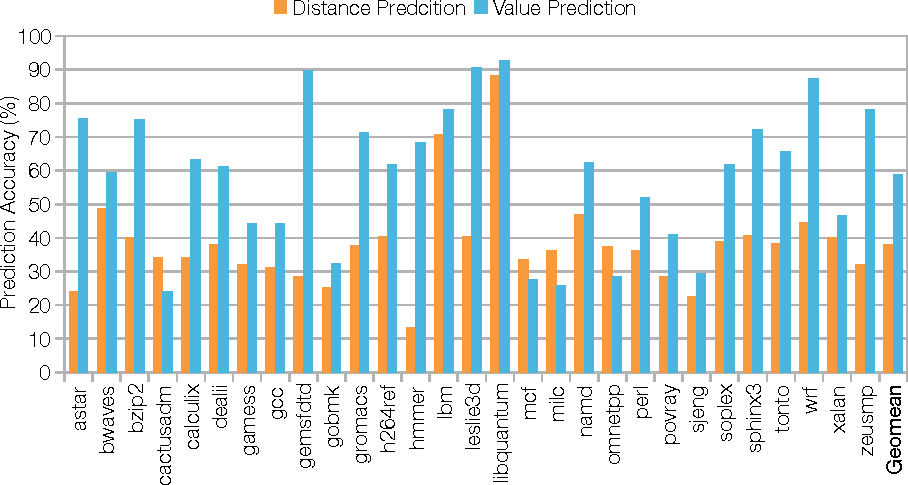
\includegraphics[width=0.50\textwidth]{graphs/DistVsValue.pdf}}
%\captionsetup{justification=centering}
\caption{Prediction accuracy of using distance and value prediction}
\label{fig:DistVsValue}
\end{figure}

\begin{figure}[ht]
\centerline{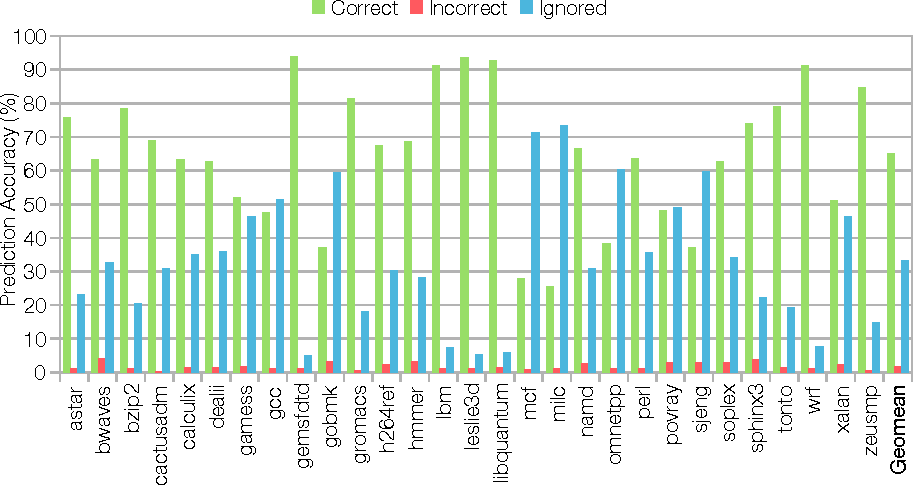
\includegraphics[width=0.50\textwidth]{graphs/ValuePredAccuracy.pdf}}
%\captionsetup{justification=centering}
\caption{Value prediction accuracy for all load addresses}
\label{fig:VPAccuracy}
\end{figure}

\subsection{Memory access reduction}

\begin{figure}[ht]
\centerline{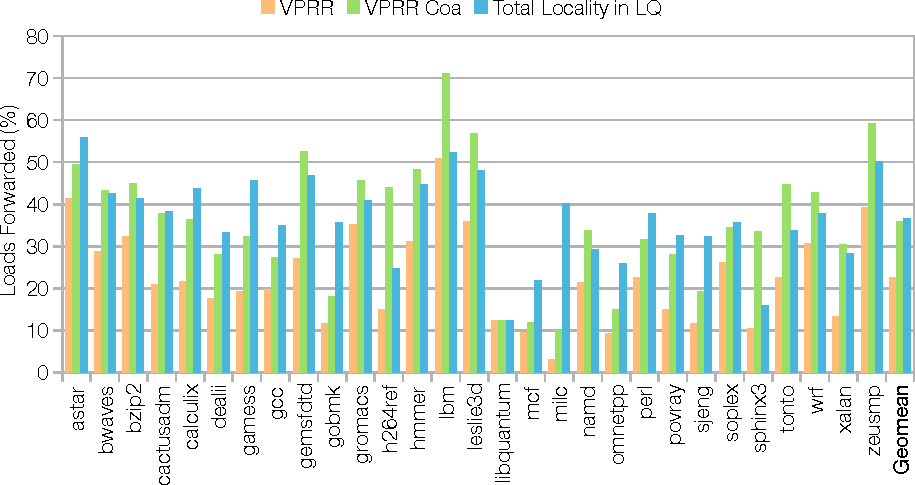
\includegraphics[width=0.50\textwidth]{graphs/RegisterReuse.pdf}}
%\captionsetup{justification=centering}
\caption{Percentage of loads that have their data forwarded from the physical register file}
\label{fig:Reuse}
\end{figure}


\begin{figure}[ht]
\centerline{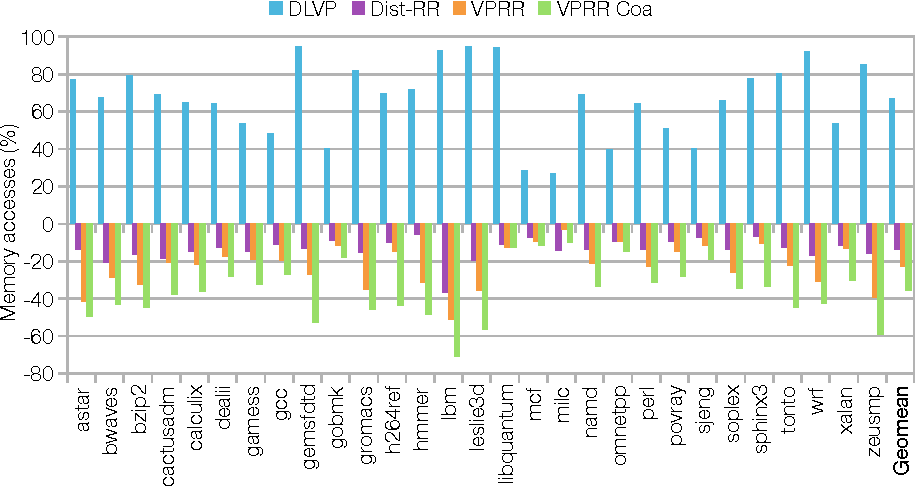
\includegraphics[width=0.50\textwidth]{graphs/MemReduction.pdf}}
%\captionsetup{justification=centering}
\caption{Percentage of loads that have their data forwarded from the physical register file}
\label{fig:MemReduction}
\end{figure}


\subsection{Performance}















\section{Conclusion}


%%%%%%%%% -- BIB STYLE AND FILE -- %%%%%%%%
\bibliographystyle{IEEEtranS}
\bibliography{refs}
%%%%%%%%%%%%%%%%%%%%%%%%%%%%%%%%%%%%

\end{document}
